Some published numerical experiments have over time become benchmarks for other codes, while some 
others showcased comparisons between codes. Here is a short list of 'famous' benchmarks' in the 
computational geodynamics community.

\begin{itemize}
\item the plastic brick \cite{lemm08,kaus10,qurj09,mishin11,maie12}
\item 2D Rayleigh-Benard convection (Blankenbach)  \cite{blbc89,trha98,chhl08,king09,lezh11,vyrc13,trab90}
\item 2D Rayleigh-Taylor convection/instability \cite{pros81,trab90,popo92,soga01,bast02,taki03,bomh06, basd08,qurj09,saev10,lezh11,vyrc13,vkks97,bomh06,chtl13,deka08,mishin11,maie12,fusc13} 
\item subduction problems \cite{scbe08,vack08,cehg14}
\item numerical sandbox \cite{bbeg06,maie12,busa16}
\item the Stokes sphere \cite{galemanual}
\item the sinking block \cite{thie11,cehg14,gery10,geyu03,mishin11,maie12}
\item 2D compressible Stokes flow problem \cite{lezh08}
\item 3D convection at infinite Prandtl number (Busse) \cite{bucc93,trha98}
\item Free surface evolution \cite{crsg12}
\item Love's problem \cite{bebe04}
\item Poiseuille flow \cite{fojg94,fuku11}
\item Couette flow
\item Poiseuille-Couette flow \cite{fusc13}
\item Lid driven Cavity \cite{foth79,bope98,kawa61}
\item Wannier flow \cite{wann50,yemu99}
\item bending of elastic plate \cite{cehg14,boht08a}
\item flexure of finite length elastic plate \cite{chtl13}
\item thermal diffusion of half-cooling space \cite{chtl13}
\item stress build-up in Maxwell visco-elastic material \cite{geyu07,chtl13}
\item plastic oedometer test  \cite{chtl13}
\item SolCx
\item SolKz
\item SolVi / inclusion \cite{kapo06,maie12,deka08}
\item channel flow (nonlinear) \cite{maie12,frbt19,gery10}
\item indentor, punch problem \cite{thfb08,mota77,gltf18}. See also \cite{hukm03,fojd04,gerb12} for application.
\item relaxation of sinusoidal topography \cite{crsg12,robh17}
\item Three-dimensional folding of an embedded viscous layer in pure shear \cite{flet91}


\end{itemize}

\todo[inline]{go through my papers and add relevant ones here}

%..................................................
\subsubsection{Relaxation of sinusoidal topography}

Following Kramer et al. \cite[Section 3.1.1]{krwd12} and \cite{robh17} 
the benchmark consists of the relaxation of surface topography in a 
two-dimensional Cartesian box with an isoviscous fluid. 
Free slip boundary conditions are imposed on the sides and bottom of the domain.
The setup is as follows:

\begin{center}
\begin{minipage}{0.45\textwidth}
\centering
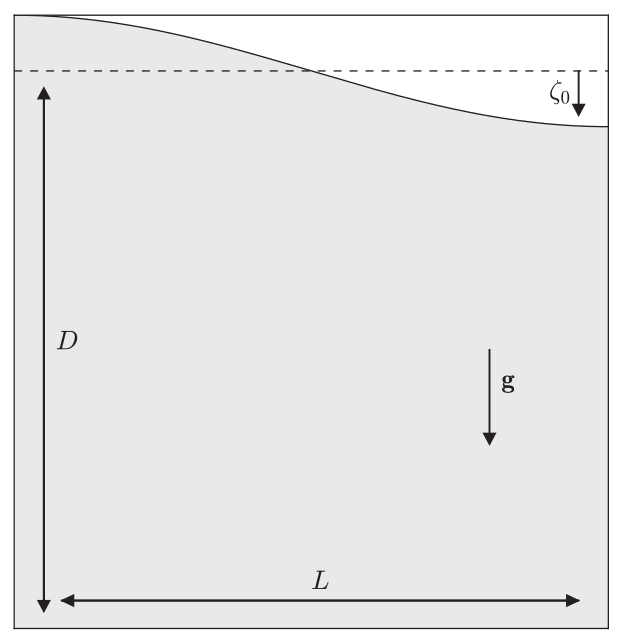
\includegraphics[height=0.8\textwidth]{images/benchmark_relaxation/robh17}\\
{\small Taken from \cite{robh17}. Setup for the free surface relaxation benchmark.
For the tests $\rho=\eta=g=L=D=1$ and $\xi_0=0.005$.}
\end{minipage}\hfill
\begin{minipage}{0.45\textwidth}
\centering
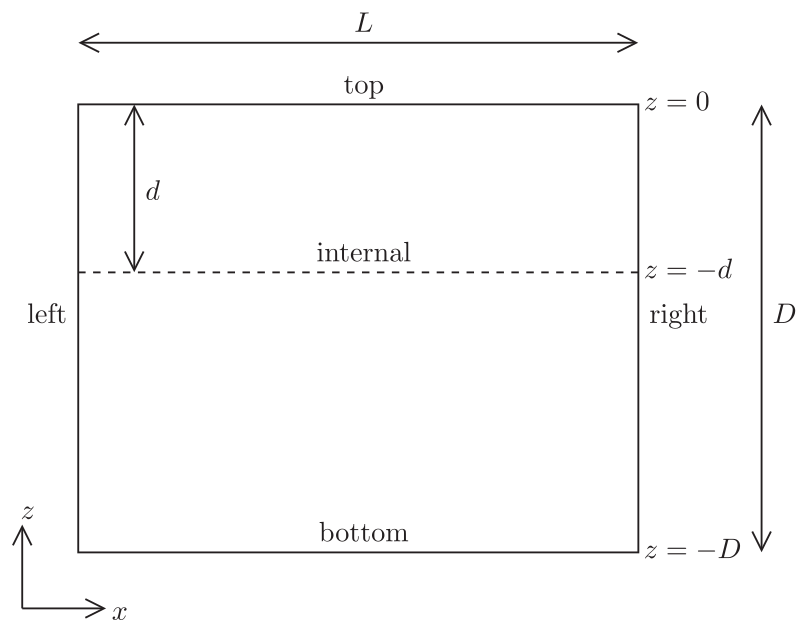
\includegraphics[height=0.8\textwidth]{images/benchmark_relaxation/krwd12}\\
{\small Taken from \cite{krwd12}. $D=3\cdot 10^6$,$\eta=10^{21}$, $\rho=4500$, $g=10$, $\xi_0=10^3$m, and 
$L=D/4,D/2,D,2D,4D$.}
\end{minipage}
\end{center}
and the infinitesimal sinusoidal perturbations to the free surface is given by
\[
\xi(x,t=0)=\xi_0 \cos \left( \frac{2 \pi n x}{L}  \right)
\]
where $n$ is a wavenumber which is an integer multiple of 1/2 (taken to be 1/2 exactly in both cases).



